\documentclass{beamer}
\usepackage[utf8]{inputenc}
\usepackage[spanish]{babel}
\usepackage{hyperref}
\usepackage{verbatim}
\usepackage{listings}
\usepackage{tikz}
\usetikzlibrary{arrows}

\setbeamercovered{invisible}
\usetheme{Frankfurt}
\usefonttheme{serif}

% Configurar los listings (Códigos)
\renewcommand{\lstlistingname}{Código}
\lstset{
	language=C++,               % Lenguaje
	basicstyle=\ttfamily\footnotesize,  % Tipo de fuente
	keywordstyle=\color{blue},  % Color de palabras clave
	stringstyle=\color{red},    % Color de strings
	commentstyle=\color{gray},  % Color de comentarios
	showstringspaces=false,     % No muestrar el _ cuando el string tiene espacios
	breaklines = true,          % Partir las líneas largas
	breakatwhitespace=true,	    % Partir las líneas en un espacio
	numbers=left,				% Numerar las líneas a la izq
	numberstyle=\tiny,			% Poner los números de las líneas pequeños
	numberblanklines=true,      % Numerar las líneas en blanco
	columns=fullflexible,       % No perder el formato al dejar los espacios
	keepspaces=true,   			% Dejar los espacios insertados
	frame=tb,					% Poner el recuadro
}

\AtBeginSection[]{%
  \begin{frame}<beamer>
    \frametitle{Contenido}
    \tableofcontents[sectionstyle=show/hide,subsectionstyle=hide/show/hide]
  \end{frame}
  \addtocounter{framenumber}{-1}% If you don't want them to affect the slide number
}

\title{Semillero de Programación}
\subtitle{Árbol de mínima expansión}
\author{Ana Echavarría \and Juan Francisco Cardona}

\institute{Universidad EAFIT}
\date{19 de abril de 2013}

\begin{document}

\begin{frame}
	\titlepage
\end{frame}

\begin{frame}
	\frametitle{Contenido}
	\tableofcontents
\end{frame}

\section{Problemas semana anterior}
	\subsection{Problema A - Minesweeper}
	
	\begin{frame}
		\frametitle{Problema A - Minesweeper}
		Para cada una de las celdas que no tienen minas, recorrer las 8 celdas adyacentes y contar el número de esas celdas que tengan una mina.
	\end{frame}
	
	\begin{frame}[fragile, allowframebreaks]
		\frametitle{Implementación}
		\begin{lstlisting}
			string board [105];
			int rows, cols;

			int di [] = {-1, -1, -1, +0, +0, +1, +1, +1};
			int dj [] = {-1, +0, +1, -1, +1, -1, +0, +1};

			bool in(int i, int j){
			    if (i >= 0 and i < rows and j >= 0 and j < cols) return true;
			    return false;
			}

			void solve (){
			    for (int i = 0; i < rows; i++){
			        for (int j = 0; j < cols; j++){
			            if (board[i][j] == '.') board[i][j] = '0';
			        }
			    }

			    for (int i = 0; i < rows; i++){
			        for (int j = 0; j < cols; j++){
			            if (board[i][j] == '*') continue;
			            for (int k = 0; k < 8; k++){
			                int next_i = i + di[k];
			                int next_j = j + dj[k];
			                if (!in(next_i, next_j)) continue;
			                if (board[next_i][next_j] == '*'){
			                    board[i][j]++;
			                }
			            }
			        }
			    }

			    for (int i = 0; i < rows; i++){
			        for (int j = 0; j < cols; j++){
			            printf("%c", board[i][j]);
			        }
			        puts("");
			    }
			}


			int main(){
			    int run = 1;
			    while (cin >> rows >> cols){
			        if (rows == 0 and cols == 0) break;
			        if (run != 1) printf("\n");
			        for (int i = 0; i < rows; i++){
			            cin >> board[i];
			        }

			        printf("Field #%d:\n", run++);
			        solve();
			    }
			    return 0;
			}
		\end{lstlisting}
	\end{frame}
	
	\subsection{Problema B - The Tourist Guide}
	\begin{frame}
		\frametitle{Problema B - The Tourist Guide}
		\begin{itemize}
			\item Hallar el camino entre la ciudad $s$ y la $d$ que pueda transportar el mayor número de personas posible.
			\item De todos los caminos entre $s$ y $d$ hay que hallar el que la ruta de bus que pueda transportar menos gente sea lo más grande posible.
			\item En otras palabras, hay que hallar el camino cuya mínima arista sea lo más grande posible (maximin).
		\end{itemize}
	\end{frame}
	
	\begin{frame}
		\begin{itemize}
			\item Luego de hallar la capacidad de dicha ruta hay que ver cuántos viajes hay que hacer teniendo en cuenta que el guía debe estar en cada viaje.
			\item Esto implica que en realidad la capacidad es 1 menor (el puesto que ocupa el guía).
			\item El número de viajes que hay que hacer es el techo de la división entre el número de pasajeros y la capacidad de la ruta.
		\end{itemize}
		\begin{block}{Función techo}
			$\displaystyle \left\lceil \frac{a}{b} \right\rceil = \left\lfloor \frac{a + b - 1}{b} \right\rfloor = \left\lfloor \frac{a - 1}{b} \right\rfloor + 1$
		\end{block}
	\end{frame}
	
	\begin{frame}[fragile, allowframebreaks]
		\frametitle{Implementación}
		\begin{lstlisting}
			const int MAXN = 105;
			const int INF = 1 << 30;
			int g[MAXN][MAXN];

			int main(){
			   int n, m;
			   int scenario = 1;
			
			   while (cin >> n >> m){
			      if (n == 0 and m == 0) break;
			
			      for (int i = 0; i <= n; ++i){
			         for (int j = 0; j <= n; ++j){
			            g[i][j] = -INF;
			         }
			         g[i][i] = INF;
			      }



			      for (int i = 0; i < m; ++i){
			         int u, v, p;
			         cin >> u >> v >> p;
			         u--; v--;
			         g[u][v] = g[v][u] = p;
			      }

			      for (int k = 0; k < n; ++k){
			         for (int i = 0; i < n; ++i){
			            for (int j = 0; j < n; ++j){
			               g[i][j] = max(g[i][j], min(g[i][k] , g[k][j]));
			            }
			         }
			      }



			      int s, d, t;
			      cin >> s >> d >> t;
			
			      // Recordar que el guia debe viajar en el bus
			      int max_cap = g[s-1][d-1] - 1;
			      // Tomar el techo de la division
			      int trips = (t + max_cap - 1) / max_cap;

			      printf("Scenario #%d\n", scenario++);
			      printf("Minimum Number of Trips = %d\n\n", trips);
			   }
			    return 0;
			}
		\end{lstlisting}
	\end{frame}
	
	\subsection{Problema C - Page Hopping}
	\begin{frame}
		\frametitle{Problema C - Page Hopping}
		\begin{itemize}
			\item Los nodos pueden no ser consecutivos, usar un mapa para guardarlos.
			\item Hallar la distancia más corta entre cualquier para de nodos.
			\item Para cada nodo, sumar la distancia a los demás $n-1$ nodos.
			\item Para sacar el promedio, dividir entre el número de distancias sumadas $n * (n-1)$.
		\end{itemize}
		
	\end{frame}
	
	
	\begin{frame}[fragile, allowframebreaks]
		\frametitle{Implementación}
		\begin{lstlisting}
			const int MAXN = 105;
			const int INF = 1 << 25;
			map <int, int> m;
			int d[MAXN][MAXN];

			int main(){
			   int run = 1;

			   int a, b;
			   while(cin >> a >> b){
			      if (a == 0 and b == 0) break;

			      for (int i = 0; i < MAXN; ++i) {
			         for (int j = 0; j < MAXN; ++j){
			            d[i][j] = INF;
			         }
			         d[i][i] = 0;
			      }
			      m.clear();

			      int node_count = 0;
			      do{
			         if (m.count(a) == 0) m[a] = node_count++;
			         if (m.count(b) == 0) m[b] = node_count++;
			         d[m[a]][m[b]] = 1;
			         cin >> a >> b;
			      }while(a != 0 or b != 0);

			      for (int k = 0; k < node_count; ++k){
			         for (int i = 0; i < node_count; ++i){
			            for (int j = 0; j < node_count; ++j){
			               d[i][j] = min(d[i][j], d[i][k] + d[k][j]);
			            }
			         }
			      }


			      int sum = 0;
			      for (int i = 0; i < node_count; ++i){
			         for (int j = 0; j < node_count; ++j){
			            sum += d[i][j];
			         }
			      }
			      // Multiplicar por 1.0 para convertir a doble y hacer           division decimal
			      double ans = 1.0 * sum / (node_count * (node_count - 1));
			      // Imprimir con tres decimales de precision
			      printf("Case %d: average length between pages = %.3lf               clicks\n", run++, ans);

			   }
			    return 0;
			}
			
		\end{lstlisting}
	\end{frame}


\section{Árboles}

	\begin{frame}
		\frametitle{Árboles}
		\begin{block}{Árboles}
			Un árbol es un grafo \textbf{no dirigido, conexo, y no cíclico}.\\
			Un grafo no dirigido y no cíclico pero no necesariamente conexo (todos los nodos están conectados) es un bosque.
		\end{block}
		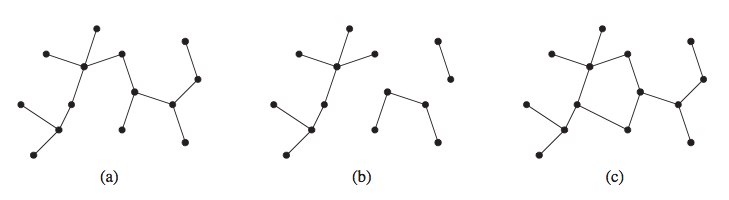
\includegraphics[width = 1\textwidth]{Tree.png}
	\end{frame}
	
	\begin{frame}
		\frametitle{Propiedades de los árboles}
		\begin{block}{Propiedades}
			Sea $G = (V, E)$ un grafo no dirigido. Los siguientes enunciados son equivalentes:
			\begin{itemize}
				\item $G$ es un árbol
				\item Hay un único camino entre cualquier par de nodos $u, v \in V$
				\item $G$ es un grafo conexo y $|E| = |V| - 1$
			\end{itemize}
		\end{block}
	\end{frame}
	
	\begin{frame}
		\frametitle{Árboles con raíces}
		Un árbol $T = (V, E)$ en donde se decide diferenciar uno de sus nodos es un árbol con raíz (rooted tree). El nodo $r$ que se diferencia de los demás se llama raíz.\\
		\begin{center} 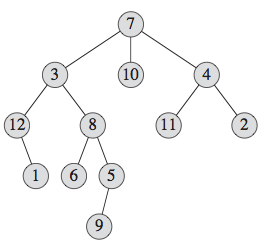
\includegraphics[height = 0.55\textheight]{RootedTree.png}  \end{center}
	\end{frame}
	
	\begin{frame}
		\frametitle{Árboles con raíces}
		Sea $T = (V, E)$ un árbol con raíz $r \in V$. Sean $x, y \in V$. \\ \quad \\
		\begin{itemize}
			\item Cualquier nodo $y$ que pertenezca al camino de $r$ a $x$ (recordemos que sólo hay un camino) es llamado \textbf{ancestro} de $x$ y $x$ a su vez es llamado \textbf{descendiente} de $y$.
			\item Si $y$ es el último nodo en el camino de $r$ a $x$, $y$ es llamado \textbf{padre} de $x$ y $x$ es llamado \textbf{hijo} de $y$.
			\item Si dos nodos tienen el mismo padre estos son llamados \textbf{hermanos}.
			\item Un nodo que no tiene hijos es llamado \textbf{hoja}.
		\end{itemize}
	\end{frame}
	
	\begin{frame}[fragile]
		\frametitle{Árboles binarios}
		Un árbol binario $T$ es un árbol con raíz en el que todos sus nodos tienen 0, 1 o 2 hijos.\\
		Los árboles binarios tienen gran aplicación en las estructuras de datos.\\
		Algunas estructuras de datos que utilizan árboles binarios para almacenar sus datos son: set, map y heap (\verb|priority_queue|).
		\begin{center} 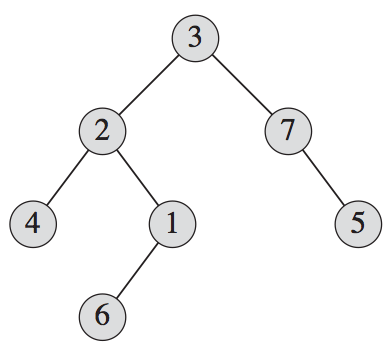
\includegraphics[height = 0.4\textheight]{BinaryTree.png}  \end{center}
	\end{frame}


\section[MST]{Minimum Spanning Tree}
	\begin{frame}
		\frametitle{Minimum Spanning Tree}
		\textcolor{blue}{\large Entrada}\\
		Un grafo $G = (V, E)$ no dirigido y conexo\\ 
		Una función de pesos $w(u, v)$ donde $(u, v) \in E$ \\ \quad \\
		\textcolor{blue}{\large Objetivo}\\
		Hallar un conjunto no cíclico $T \subseteq E$ que conecte todos los nodos de $G$ y que minimice su peso
		$$w(T) = \sum_{(u, v) \in T}{w(u, v)}$$
		Ya que $T$ es no cíclico, conexo y no dirigido, es un árbol y es llamado el \textbf{árbol de mínima expansión}.
	\end{frame}
		
	\begin{frame}
		\frametitle{Minimum Spanning Tree}
		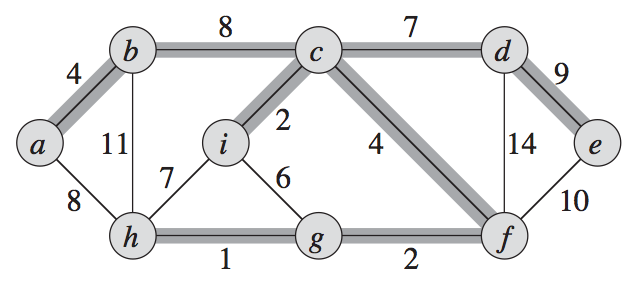
\includegraphics[width = \textwidth]{MST.png}
	\end{frame}
	

\section[Prim]{Algoritmo de Prim}
	\begin{frame}
		\frametitle{Algoritmo de Prim}
		\begin{enumerate}
			\item{Seleccionar un nodo al azar y agregarlo al conjunto de visitados}
			\item{Mientras que haya nodos sin visitar}
			{\setlength\itemindent{15pt} \item Tomar la arista con menor peso que conecte un nodo visitado $u$ y uno no visitado $v$}
			{\setlength\itemindent{15pt} \item Agregar la arista $(u, v)$ al MST}
			{\setlength\itemindent{15pt} \item Agregar $v$ al conjunto de visitados}
		\end{enumerate}
	\end{frame}
	
	\begin{frame}
		\frametitle{Ejemplo}
		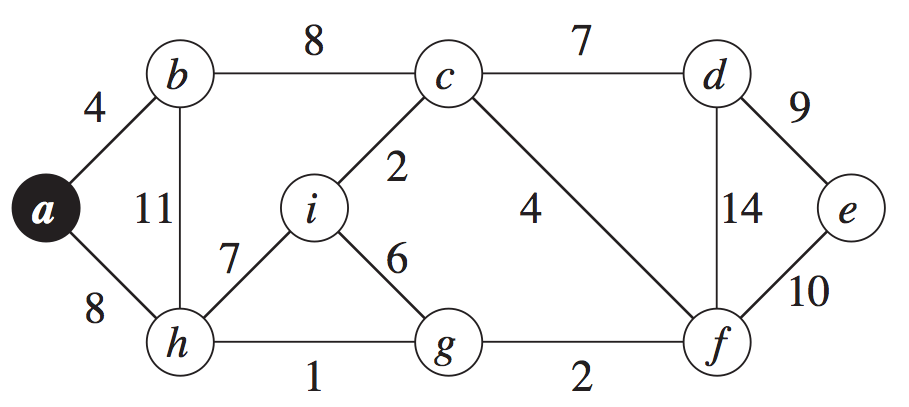
\includegraphics[width = \textwidth]{Ejemplo.png}
	\end{frame}
	
	\begin{frame}
		\frametitle{¿Por qué funciona?}
		Veamos que el grafo que el algoritmo produce es un árbol.
		\begin{itemize}
			\item En cada iteración, se agrega al grafo un nodo nuevo y una arista que conecta a ese nodo con alguno de los ya elegidos anteriormente. Al final se tendrán todos los nodos conectados.
			\item Nunca se agrega una arista que una a dos nodos ya elegidos por lo que no se generan ciclos.
			\item Por las dos afirmaciones anteriores se puede concluir que el algoritmo produce un árbol.
		\end{itemize}
		La prueba de optimalidad sale de un teorema que dice que la mínima arista que cruza una partición de un grafo en dos grupos siempre está en el MST de ese grafo.
	\end{frame}
	
	\begin{frame}
		\frametitle{Optimización}
		En el algoritmo de Prim se necesita extraer el mínimo de un arreglo repetidas veces. ¿Cómo hacer esto rápidamente?\\ \quad \\
		\pause
		Estos llamados se pueden hacer rápidamente utilizando un \textbf{heap} como se hizo en el algoritmo de Dijkstra.
	\end{frame}
	
	\begin{frame}[fragile, allowframebreaks]
		\frametitle{Implementación}
		\begin{lstlisting}
			const int MAXN = 10005;
			typedef pair <int, int> edge;
			bool visited[MAXN];
			// g[i] = lista de parejas (nodo, peso)
			vector <pair <int, int> > g[MAXN]; 

			int prim(int n){
			    for (int i = 0; i <= n; ++i) visited[i] = false;
			    int total = 0;
			    // Crear el heap de forma que se extraiga el de menor peso
			    // El heap es de parejas (peso, nodo), contrario al grafo
			    priority_queue<edge, vector <edge>, greater<edge> > q;
			    // Empezar el MST desde el nodo 0
			    q.push(edge(0, 0));
			    while (!q.empty()){
			        int u = q.top().second;
			        int w = q.top().first;
			        q.pop();
			        // Si es una arista entre dos nodos ya incluidos al MST
			        if (visited[u]) continue;

			        visited[u] = true;
			        total += w;
			        for (int i = 0; i < g[u].size(); ++i){
			            int v = g[u][i].first;
			            int next_w = g[u][i].second;
			            // Si v no pertenece todavia al MST
			            if (!visited[v]){
			                // Insertar primero el peso y luego el nodo
			                q.push(edge(next_w, v));    
			            }    
			        }
			    }
			    return total; // El costo total del MST
			}
		\end{lstlisting}
	\end{frame}
	
	\begin{frame}
		\frametitle{Complejidad}
		\begin{block}{Complejidad}
			El algoritmo de Prim implementado con un heap tiene una complejidad de $O(E\operatorname{log} V)$
		\end{block}
	\end{frame}

\section[Union-Find]{Union-Find}
	\begin{frame}[fragile]
		\frametitle{Union-Find}
		Union-Find es una estructura de datos para almacenar una colección conjuntos disjuntos (no tienen elementos en común) que cambian dinámicamente. \\ \quad \\
		Para hacer esto identifica en cada conjunto un ``padre'' que es un elemento al azar de ese conjunto y hace que todos los elementos del conjunto ``apunten'' hacia ese padre. \\ \quad \\
		Inicialmente se tiene una colección donde cada elemento es un conjunto unitario.
	\end{frame}
	
	\begin{frame}
		\frametitle{Union-Find}
		Esta estructura de datos tiene dos operaciones: \\ \quad \\
		\begin{description}
			\item[Union(u, v)] Une los conjuntos que contienen a $u$ y a $v$ en un solo conjunto.
			\item[Find(u)] Retorna el padre del (único) conjunto que contiene a $u$.
		\end{description}
	\end{frame}
	
	\begin{frame}[fragile]
		\frametitle{Implementación}
		\begin{lstlisting}
			int p[MAXN]; //p[i] el padre del conjunto al que pertenece i
			
			// Inicializa los conjuntos de los elementos 0 a n
			void initialize(int n){
			    for (int i = 0; i <= n; ++i) p[i] = i;
			}
			// Retorna el padre del conjunto que contiene a u
			int find(int u){
			    if (p[u] == u) return u;
			    return p[u] = find(p[u]);
			}
			// Une los conjuntos a los que pertenecen u y v
			// Este nuevo conjunto tiene como padre el padre de v
			void join(int u, int v){
			     int a = find(u);
			     int b = find(v);
			     if (a == b) return; // Son el mismo conjunto
			     p[a] = b; // El padre del padre de u es el padre de v
			}
		\end{lstlisting}
	\end{frame}
	
	\begin{frame}[fragile]
		\frametitle{Ejemplo}
		Se tiene inicialmente una colección con 5 conjuntos $\left\{\{0\}, \{1\}, \{2\}, \{3\}, \{4\}\right\}$ y se realizan las siguientes operaciones:
		\begin{enumerate}
			\item join(0, 1)
			\item join(0, 2)
			\item join(1, 3)
			\item join(0, 4)
		\end{enumerate}
	\end{frame}
	
	\begin{frame}
		\frametitle{Complejidad}
		\begin{block}{Complejidad}
			Sean $m$ el número total de operaciones de initialize, union y find realizadas.\\
			La implementación de union-find mostrada tiene una complejidad aproximada de $O(m)$
		\end{block}
	\end{frame}

\section[Kruskal]{Algoritmo de Kruskal}
	\begin{frame}
		\frametitle{Algoritmo de Kruskal}
		El algoritmo de Kruskal utiliza Union-Find para verificar que al agregar una arista no esté generando un ciclo.
		\begin{enumerate}
			\item Ordenar las aristas de menor costo a mayor costo (desempate es indiferente)
			\item Para cada arista (u, v) en el orden de menor a mayor costo
			{\setlength\itemindent{15pt} \item Si agregar la arista $(u, v)$ no genera un ciclo}
			{\setlength\itemindent{30pt} \item Agregar la arista $(u, v)$ al MST}
		\end{enumerate}
	\end{frame}

	\begin{frame}
		\frametitle{Ejemplo}
		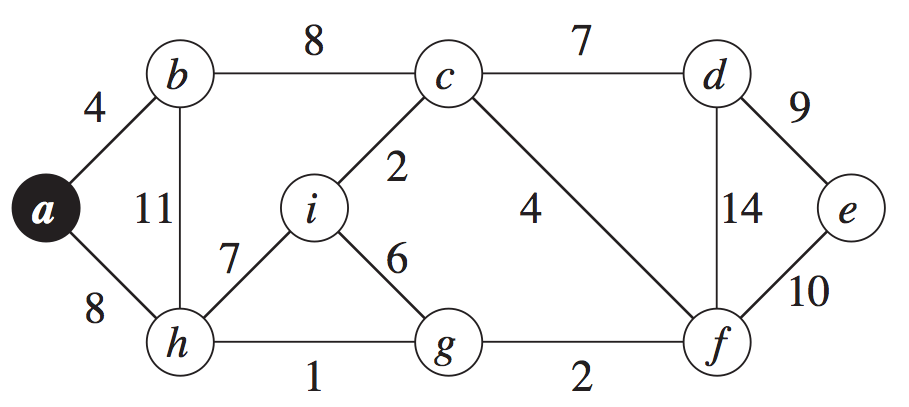
\includegraphics[width = \textwidth]{Ejemplo.png}
	\end{frame}
	
	\begin{frame}
		\frametitle{¿Por qué funciona?}
		\begin{itemize}
			\item Claramente el grafo resultante no tiene ciclos
			\item El grafo está conectado, si no lo estuviera es porque quedaron dos grupos de nodos.
			\item Estos dos grupos de nodos estaban conectados en el grafo original están conectados por al menos una arista pero estamos suponiendo que el algoritmo de Kruskal no seleccionó ninguna de esas aristas (porque quedaron los dos grupos separados)
			\item Sin embargo el algoritmo tuvo que haber seleccionado alguna de las aristas porque no generaban ningún ciclo.
			\item Por los dos afirmaciones anteriores se concluye que el algoritmo produce un árbol.
		\end{itemize}
		La prueba de optimalidad sale de que el algoritmo de Kruskal va a tomar siempre la va a tomar la mínima arista que cruza una partición del grafo porque empieza por la menor.
	\end{frame}

	\begin{frame}
		\frametitle{Optimización}
		En el algoritmo de Kruskal se necesita verificar que no se genere un ciclo repetidas veces. ¿Cómo hacer esto rápidamente?
		\pause
		\begin{itemize}
			\item A medida que se ejecuta el algoritmo de Kruskal se empiezan a unir los nodos en conjuntos disjuntos.
			\item Un ciclo se genera si se unen dos nodos que pertenecen al mismo conjunto.
			\item Se utiliza union-find para guardar el conjunto al que pertenece cada nodo.
			\item Para verificar se genera un ciclo es ver si el conjunto de $u$ es igual al conjunto de $v$.
		\end{itemize}
	\end{frame}

	\begin{frame}[fragile, allowframebreaks]
		\frametitle{Implementación}
		\begin{lstlisting}
			// Estrutura personalizada para manejar las aristas.
			// En el algoritmo de Kruskal el grafo se guarda como lista de aristas y no como lista de adyacencia
			struct edge{
			   // Atributos
			   int start, end, weight;
			   // Constructor
			   edge(int u, int v, int w){
			      start = u; end = v; weight = w;
			   }
			   // Comparador menor
			   bool operator < (const edge &other) const{
			      return weight < other.weight;
			   }
			}; // No olvidar este ;
			
			
			
			const int MAXN = 100005;
			vector <edge> edges;
			int p[MAXN];

			int find(int u){
			    if (p[u] == u) return u;         
			    return p[u] = find(p[u]);
			}

			void join(int u, int v){
			     int a = find(u);
			     int b = find(v);
			     if (a == b) return;
			     p[a] = b;  
			}
			
			
			
			
			int kruskal(int n){
			   // Inicializar el arreglo de union-find
			   for (int i = 0; i <= n; ++i) p[i] = i;
			   // Ordenar las aristas de menor a mayor
			   sort(edges.begin(), edges.end());
			
			   int total = 0;
			   for (int i = 0; i < edges.size(); ++i){
			      int u = edges[i].start;
			      int v = edges[i].end;
			      int w = edges[i].weight;
			      if (find(u) != find(v)){ // Si no genera un ciclo
			         total += w;
			         join(u, v);
			      }
			   }
			   return total;
			}
		\end{lstlisting}
	\end{frame}

	\begin{frame}
		\frametitle{Complejidad}
		\begin{block}{Complejidad}
			El algoritmo de Kruskal implementado con union-find tiene una complejidad de $O(E\operatorname{log} V)$
		\end{block}
	\end{frame}

	
\section{Tarea}
	\begin{frame}[fragile]
		\frametitle{Tarea}
		\begin{alertblock}{Tarea}
			Resolver los problemas de \url{http://contests.factorcomun.org/contests/56}
		\end{alertblock}
	\end{frame}

\end{document}